\documentclass[oneside,mtp]{iiitg}

% The iitkgp.cls class is for producing theses and dissertations
% in the CSE Department of IIITG.  You can supply
% the following optional arguments in the square brackets to
% specify the thesis type:
%
%   senior  : Produces the senior thesis preliminary pages (default)
%   phd     : Produces the PhD dissertation preliminary pages
%
% FOR ALL DEPARTMENTS, open the iiitg.cls file, go to the "Certificate Page" section
% of the main code and make appropriate changes.
%
% FOR DEPARTMENTS other than CSE open the iiitg.cls file, go to the "Title Page" section
% of the main code and make appropriate changes.
%
% The default format is appropriate for printing, with blank pages
% inserted after the preliminary pages in twoside mode so you can
% send it directly to a two-sided printer. Howev  er, for ETD
% submission the blank pages need to be removed from the final output.
% The following option does this for you:
%
%   etd     : Produces a copy with no blank pages in the preliminary section.
%             Remove this option to produce a version with blank pages inserted
%             for easy double sided printing.
%
% The rest of the class options are the same as the regular book class.
% A few to remember:
%
%   oneside : Produces single sided print layout (recommended for theses less than 50 pages)
%   twoside : Produces single sided print layout (the default if you remove oneside)
%
% The BYUPhys class provides the following macros:
%
%   \makepreliminarypages : Makes the preliminary pages
%   \clearemptydoublepage : same as \cleardoublepage but doesn't put page numbers
%                           on blank intervening pages
%   \singlespace          : switch to single spaced lines
%   \doublespace          : switch to double spaced lines
%
% --------------------------- Load Packages ---------------------------------

% The graphicx package allows the inclusion of figures.  Plain LaTeX and
% pdfLaTeX handle graphics differently. The following code checks which one
% you are compiling with, and switches the graphicx package options accordingly.





%\usepackage{setspace}
\usepackage{emptypage}
\usepackage{changepage,ifthen}
%\textwidth 6.5in
%\addtolength{\oddsidemargin}{-.5in}
%\textheight 10in
%\addtolength{\topmargin}{-1in}
\addtocounter{secnumdepth}{2}
%\setlength{\parindent}{0pt}
%\usepackage{algorithm}
%\usepackage{algorithmic}
%\usepackage{hyperref}
%\usepackage{graphicx}
\usepackage{pdfpages}
%\usepackage{epsfig}
%\usepackage{amsmath}
\usepackage{geometry}
%\usepackage{setspace}
%\usepackage{arydshln}
%\usepackage{amsmath,amssymb,verbatim,eufrak}
%\usepackage[dvips,colorlinks,bookmarksopen,bookmarksnumbered,citecolor=red,urlcolor=red]{hyperref}

%\usepackage{natbib,stfloats}
\usepackage{mathrsfs}
\usepackage{algorithm}
\usepackage{algpseudocode}
%\usepackage{fixltx2e}
%\usepackage{stfloats}
\usepackage{comment}
\usepackage{float}
%\usepackage{url}
\usepackage{arydshln}
\algtext*{EndIf}




















\usepackage{amsfonts}
\usepackage{amssymb}
\usepackage[centertags]{amsmath}
\usepackage{epsfig}
\usepackage{epstopdf}
\usepackage{enumerate}
\usepackage{graphicx}
\usepackage{graphics}
\usepackage{subfig}
\usepackage{multirow}
\usepackage{rotating}
\usepackage{times}
\usepackage{lscape}
\usepackage[bottom]{footmisc}
\usepackage{booktabs}
\usepackage{colortbl}
\usepackage{threeparttable}
\usepackage{algorithm}
\usepackage{algorithmicx}
%\usepackage[lined,algonl,algochapter,algoruled]{algorithm2e}
\usepackage{algpseudocode}
\usepackage{amsthm}
\usepackage{epstopdf}
%\usepackage[cmex10]{amsmath}
%\usepackage{hyperref}
\usepackage{graphicx}


\usepackage{geometry}

\usepackage{fixltx2e}








 








\newcommand {\g}[1]{\textcolor[gray]{0.6} {#1}}
\newcommand{\todo}[1]{\textcolor{red}{TODO: #1}\\}
\newcommand{\done}[1]{\textcolor{blue}{Tried to address. #1}\\}

% these are for the algorithms style file, for writing algorithms
\renewcommand{\algorithmicrequire}{\textbf{Input:}}
\renewcommand{\algorithmicensure}{\textbf{Output:}}
%\renewcommand{\algorithmiccomment}[1]{\begin{small}/* #1 */\end{small}}
\renewcommand{\algorithmiccomment}[1]{/* #1 */}

% The fancyhdr package allows you to easily customize the page header.
% The settings below produce a nice, well separated header.
\usepackage{fancyhdr}
  \fancyhead{}
  \fancyhead[LO]{\slshape \rightmark}
  \fancyhead[RO,LE]{\textbf{\thepage}}
  \fancyhead[RE]{\slshape \leftmark}
  \fancyfoot{}
  \pagestyle{fancy}
  \renewcommand{\chaptermark}[1]{\markboth{\chaptername \ \thechapter \ \ #1}{}}
  \renewcommand{\sectionmark}[1]{\markright{\thesection \ \ #1}}

% The caption package allows us to change the formatting of figure captions.
% The commands here change to the suggested caption format: single spaced and a bold tag
% Change the \DeclareCaptionFormat line below to make the captions fully bold
\usepackage{caption}
%\DeclareCaptionFormat{suggested}{\singlespace#1#2 #3\par\doublespace}
\DeclareCaptionFormat{suggested}{\singlespace \textbf{#1}\textbf{#2}#3 \doublespace}
\captionsetup{format=suggested}

%To instruct Latex to try to fit each paragraph into 1 less line
%\let\markeverypar\everypar
%\newtoks\everypar
%\everypar\markeverypar
%\markeverypar{\the\everypar\looseness=-1\relax}

%\newcommand{\captionfonts}{\small}

% The cite package cleans up the way citations are handled.  For example, it
% changes the citation [1,2,3,6,7,8,9,10,11] into [1-3,6-11].  If your advisor
% wants superscript citations, use the overcite package instead of the cite package.
\usepackage{cite}
%\usepackage[tone]{tipa}

% The makeidx package makes your index for you.  To make an index entry,
% go to the place in the book that should be referenced and type
%  \index{key}
% An index entry labeled "key" (or whatever you type) will then
% be included and point to the correct page.
\usepackage{makeidx}
\makeindex

\usepackage[hyphens]{url}
\urlstyle{rm}

% If you have a lot of equations, you might be interested in the amstex package.
% It defines a number of environments and macros that are helpful for mathematics.
% We don't do much math in this example, so we haven't used amstex here.
%
% To include a link in your pdf use \href{URL}{Text to be displayed}.  If your
% display text is the URL, you probably should use the \url{} command discussed
% above.
%
% To add a bookmark in the pdf you can use \pdfbookmark.  You can look up its usage
% in the hyperref package documentation
\usepackage[bookmarksnumbered,pdfpagelabels=true,plainpages=false,colorlinks=true,
            linkcolor=black,citecolor=black,urlcolor=blue]{hyperref}
\usepackage[hyphenbreaks]{breakurl}

% ---------------- Fill in these fields for the preliminary pages -------------------
%
% For Senior and honors this is the year and month that you submit the thesis
% For Masters and PhD, this is your graduation date

\newcommand{\bigsize}{\fontsize{14pt}{20pt}\selectfont}

\Year{2020}
\Month{April}
\Author{AAAAAA}
\degree{Master of Technology}
% If you have a long title, split it between two lines. The \TitleBottom field defines the second line
% A two line title should be an "inverted pyramid" with the top line longer than the bottom.
\TitleTop{{\bigsize \bf Anomaly Detection in Cloud Computing}}
%\TitleBottom{{\bigsize \bf  MEMORY SYSTEMS }}
%\TitleBottomagain{{\bigsize \bf MEMORY SYSTEMS}}
% Your research advisors
\AdvisorA{{Dr AAAA AAAA}}


%%%%%%%%%%%%%%%%%%%%%%%%%%%%%%%%%%%%%%%%%%%%%%%%%%%%%%%%%%%%%%%%%%%%%%%%%%%%
%%%%%%%%%%%%%%%%%%%% APPROVAL BY DSC %%%%%%%%%%%%%%%%%%%%%%%%%%%%%%%%%%%%%%%
%%%%%%%%%%%%%%%%%%%%%%%%%%%%%%%%%%%%%%%%%%%%%%%%%%%%%%%%%%%%%%%%%%%%%%%%%%%%
%
%\Approval{
%\singlespace
%\hspace{6cm}
%%Date:\hspace{.8cm}$\backslash \ \ \ \ \  \ \backslash$ 20  \\  \\
%Date:\hspace{.8cm}$/ \ \ \ \ \  \ /$ 20  \\  \\
%Certified that the thesis entitled {\bf ``TITLE OF THE THESIS''} submitted by NAME OF THE AUTHOR to the Indian Institute of Information Technology Guwahati, for the award of the degree of Master of Technology has been accepted by examiners and that the student has successfully defended the thesis in the viva-voce examination held today.
%
%\vspace{0.5in}
%
%%\noindent
%%Signature:~~~~~~~~~~\hfill Signature:~~~~~\hfill Signature:\hfill~
%
%%\noindent
%%Name:~~~~~~~~~~~~~~~\hfill Name:~~~~~~~~~~\hfill Name:~~~~~\hfill~
%
%\vspace{1in}
%\noindent
%(Member)~~~~~\hfill(Member)~~~~~\hfill(Member)
%
%\vspace{0.3in}
%%\hspace{2cm}
%%Signature:
%\vspace{1in}
%%\hspace{2cm}
%%Name:
%\noindent
%%\hspace{2cm}
%(Supervisor) %~~~~~\hfill(Supervisor 2)
%
%
%
%\vspace{0.3in}
%
%%\hspace{2cm}
%%Name:~~~~~~~~~~~~~~~~~~~~~~~\hfill Name:~~~~~\hfill ~~~~
%
%%\vspace{1in}
%%%\hspace{2cm}
%%\noindent
%%(External Examiner)\hspace{0.8in}(Chairman)
%}

%%%%%%%%%%%%%%%%%%%%%%%%%%%%%%%%%%%%%%%%%%%%%%%%%%%%%%%%%%%%%%%%%%%%%%%%%%%
%%%%%%%%%%%%%%%%%%% CERTIFICATE BY SUPERVISOR %%%%%%%%%%%%%%%%%%%%%%%%%%%%%
%%%%%%%%%%%%%%%%%%%%%%%%%%%%%%%%%%%%%%%%%%%%%%%%%%%%%%%%%%%%%%%%%%%%%%%%%%%

\Certificate{
%\noindent%
{\em This is to certify that the thesis entitled {\bf ``Anomaly detection in cloud computing''}, submitted by {\bf name} to the institute name, for the award of the degree of Master of Technology, is a record of bona fide research work carried out by him under my supervision and guidance.
The thesis, in my opinion, is worthy of consideration for the award of the degree of Master of Technology in accordance with the regulations  of the Institute.  To the best of my/our knowledge, the results embodied in the thesis have not been submitted to any other university or institute for the award of any other degree or diploma.}
% To the best of my knowledge, the results embodied in this thesis have not been submitted to any other University or Institute for the award of any other Degree or Diploma.}

\signaturebox{Dr guide name,\\ Assistant Professor,\\Department of Computer Science and Engineering\\institute name}
%\hspace{10pt}
%\signaturebox{Name of the Supervisor 2,\\ Designation,\\Department of Computer Science and Engineering\\IIIT Guwhati}

\datebox
   %\vskip 0pt plus 2fill
    %\noindent Accepted for the Department\hfill%
    %\signaturebox{\@DepRep, \@DepRepTitle\\Department of Physics and
    %Astronomy }{} \vfill \noindent Accepted for the College\hfill
    %\signaturebox{\@Dean, \@DeanTitle \\
    %College of Mathematics and Physical Sciences}

}

%%%%%%%%%%%%%%%%%%%%%%%%%%%%%%%%%%%%%%%%%%%%%%%%%%%%%%%%%%%%%%%%%%%%%%%%%%%
%%%%%%%%%%%%%%%%%%% DECLARATION BY STUDENT %%%%%%%%%%%%%%%%%%%%%%%%%%%%%%%%
%%%%%%%%%%%%%%%%%%%%%%%%%%%%%%%%%%%%%%%%%%%%%%%%%%%%%%%%%%%%%%%%%%%%%%%%%%%

\Declaration{
\noindent
I certify that
\begin{enumerate}
\item[a.]   The work contained in this thesis is original and has been done by me under 
the general supervision of my supervisor(s).
\item[b.]   The work has not been submitted to any other Institute for any degree or diploma.
\item[c.]   I have followed the guidelines provided by the Institute in writing the thesis.
\item[d.]   I have conformed to the norms and guidelines given in the Ethical Code of Conduct of the Institute.
\item[e.]   Whenever I have used materials (data, theoretical analysis, figures, and text) from other sources, I have given due credit to them by citing them in the text of the thesis and giving their details in the references.
\item[f.]   Whenever I have quoted written materials from other sources, I have put them under quotation marks and given due credit to the sources by citing them and giving required details in the references.
\end{enumerate}

\vspace{0.6in}

\hfill (Candidate name) ~ ~ ~
}

%%%%%%%%%%%%%%%%%%%%%%%%%%%%%%%%%%%%%%%%%%%%%%%%%%%%%%%%%%%%%%%%%%%%%%%%%%%
%%%%%%%%%%%%%%%%%%% ACKNOWLEDGMENTS %%%%%%%%%%%%%%%%%%%%%%%%%%%%%%%%%%%%%%%
%%%%%%%%%%%%%%%%%%%%%%%%%%%%%%%%%%%%%%%%%%%%%%%%%%%%%%%%%%%%%%%%%%%%%%%%%%%

\Acknowledgments{
\noindent



\vspace{0.5in}

\noindent
 Anomaly detection has crucial significance in the wide variety of domains as it provides critical and actionable information. For example, an anomaly in MRI image scan could be an indication of the malignant tumor or anomalous reading from production plant sensor may indicate faulty component.This thesis studies in detail various kind of anomaly detection techniques and compares them based on their effectiveness. Algorithms have been implemented in Python mostly.

I would like to thank my supervisor <> for helping me to carry out this thesis under his guidance. I am also thankful to our Head of Department Dr Rakesh Matam Sir for his valuable guidance from time to time.I would also like to thank our thesis panel based on their reivews and suggestions I improved the the work carried out.His guidance helped me in researching and writing the thesis.

\medskip
\bigskip\medskip
}

%%%%%%%%%%%%%%%%%%%%%%%%%%%%%%%%%%%%%%%%%%%%%%%%%%%%%%%%%%%%%%%%%%%%%%%%%%%
%%%%%%%%%%%%%%%%%%% ABSTRACT %%%%%%%%%%%%%%%%%%%%%%%%%%%%%%%%%%%%%%%%%%%%%%
%%%%%%%%%%%%%%%%%%%%%%%%%%%%%%%%%%%%%%%%%%%%%%%%%%%%%%%%%%%%%%%%%%%%%%%%%%%

 %The text of your abstract
\Abstract{
In today’s world of changing technologies due to advancement of technology,more and more organizations are shifting to usage off cloud computing services worldwide. With cloud computing service provider companies like Google, Amazon, AliBaba, Microsoft ,IBM  investing more and more in cloud computing.It is becoming target of internet threats, such as malware or virus, technical vulnerability and negligent behaviours.
Hence anomaly detection in cloud has been an emerging area of research for researchers like us. This thesis  addresses the main security and privacy issues in Cloud Computing. It is essential to have an Anomaly Detection System (ADS) to detect anomalies with a high detection accuracy in cloud environment. With the evolving technological setup this work becomes complex day by day. This work proposes an anomaly detection system at the administrator level to improve the accuracy of the detection system. 
The proposed system is implemented and it uses classifiers and data mining techniques to detect anomalies in network. The DARPA’s KDD cup data-set 1999 is used for experiments.  Using simple data analytics techniques the system is able to find out anomalies in cloud.
Machine Learning has various  applications: classification, predicting next value, anomaly detection, and discovering structure. In this thesis we have studied,how anomaly detection detects anomalies from security perspective on cloud service providers. Anomaly detection has a wide range of applications such as fraud detection, surveillance, diagnosis, data cleanup, and predictive maintenance.
}

\fussy

\newtheorem{thm}{Theorem}[section]
\newtheorem{cor}[thm]{Corollary}
\newtheorem{lem}[thm]{Lemma}


\normalsize
\renewcommand{\baselinestretch}{1.0}
%\newfloatcommand{capbtabbox}{table}[][\FBwidth]
%\floatsetup[table]{capposition=top}
%\graphicspath{ {/home/arya/Desktop/synopsis_seminar/figures/} }
\graphicspath{ {./figures/} }


\begin{document}
 % Start page counting in roman numerals
 \frontmatter

 % This command makes the formal preliminary pages.
 % You can comment it out during the drafting process if you want to save paper.

\makepreliminarypages

 \singlespace
 
 \clearemptydoublepage
\thispagestyle{empty}

 \hspace{-0.4cm}{\huge \textbf{List of Abbreviations}}\\
 %  \end{center}
\begin{table} [h]
%\small
%\scriptsize 
\begin{tabular}{l l}  
		\textbf{IIITG} & Indian Institute of Information Technology\\ 
		\textbf{CSE} & Computer Science and Engineering\\
		\textbf{PhD} & Doctor of Philosophy\\
		\textbf{VM} & Virtual Machine\\
		\textbf{GCP} & Google Cloud Platform\\
		\textbf{AWS} & Amazon Web Services\\
\end{tabular}
\end{table} 

\clearemptydoublepage
\thispagestyle{empty}

 \hspace{-0.4cm}{\huge \textbf{List of Symbols}}\\
 %  \end{center}
\begin{table} [h]
%\small
%\scriptsize 
\begin{tabular}{c l}
		\hline
		\textbf{Symbol} & \textbf{Description}  \\
		\hline
		$\beta$ & intensity factor\\ 
		$\alpha$ & threshold value\\
		\hline
	\end{tabular}
\end{table} 

\clearemptydoublepage
%\makepreliminarypages
 % Make the table of contents.
 \tableofcontents
 
 \clearemptydoublepage

 % Make the list of figures
 \listoffigures
 \clearemptydoublepage

 % Make the list of tables
% \listoftables (ये गायब किया )है 
 %\clearemptydoublepage (ये गायब किया )

%\phantomsection \addcontentsline{toc}{chapter}{List of Symbols and Abbreviation}
%\include{files/symb_b}
%\include{files/symb_b1}
%\clearemptydoublepage

%\onehalfspace (ये गायब किया )

 % Start regular page counting at page 1
\mainmatter
\addtolength{\parskip}{0.05\baselineskip}

\abovedisplayskip=13pt
\belowdisplayskip=13pt

\clearemptydoublepage
\input{texfiles/Chapter1}
\clearemptydoublepage

\chapter{Literature Review}
\label{chap:chapter2}
Anomaly detection covers numerous things in cloud computing from security perspective. In order to understand them, the underlying concepts that might identify the source of vulnerabilities and threats must be understood. This section analyses those concepts, starting with an explanation on virtualization elements and then on multi-tenancy. Cloud services are also discussed, followed by the discussion of the concept of service providing in cloud  and the section ends with a discussion on anomaly detection.
\begin{figure}
    \centering
    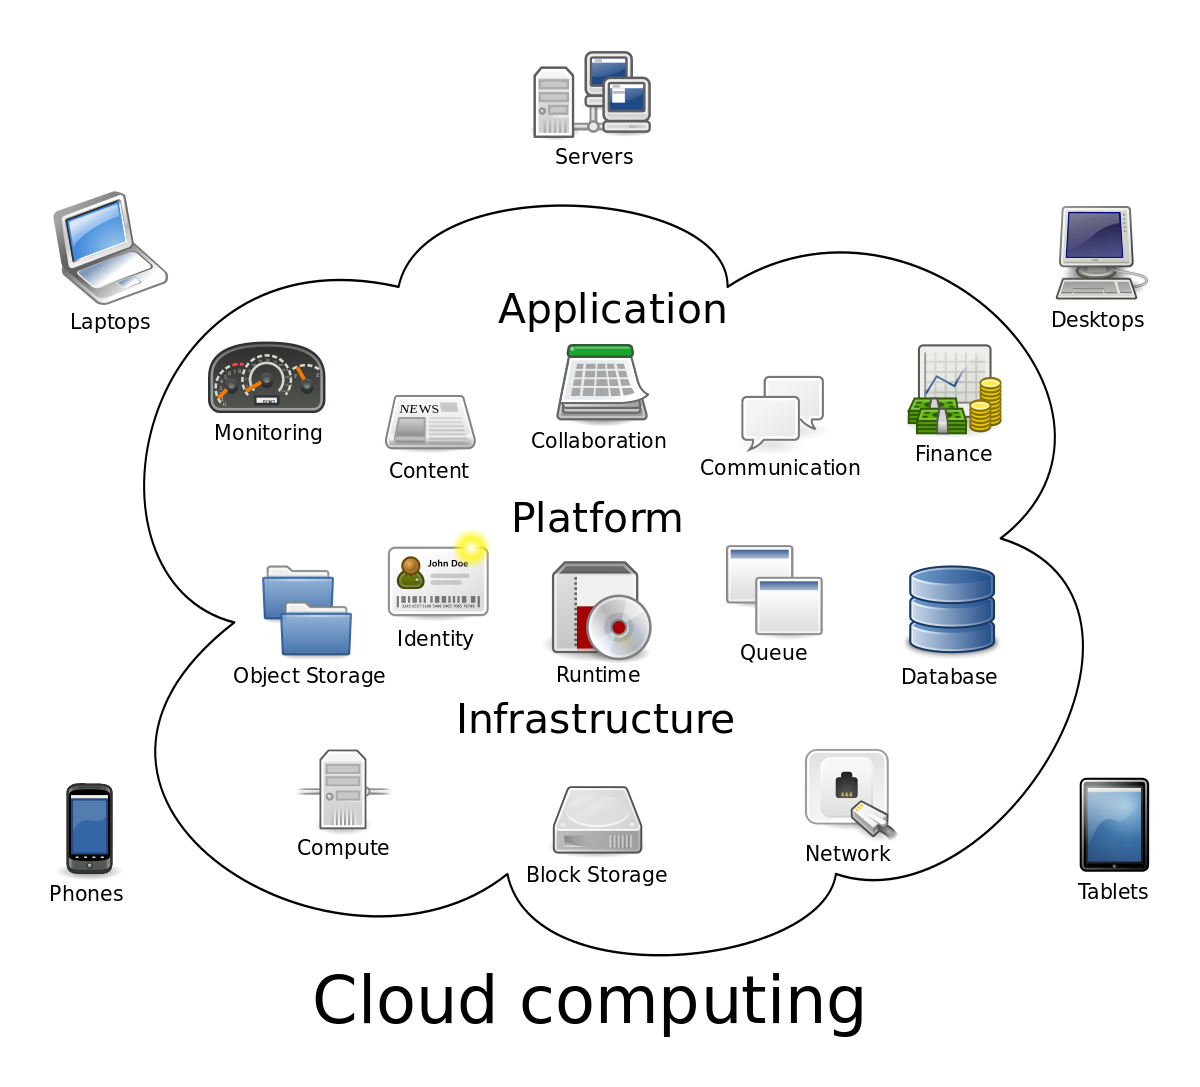
\includegraphics[width=10cm]{texfiles/images/Cloud_computing.png}
    \caption{Cloud Computing\cite{cloud33}}
    \label{fig:my_label}
\end{figure}
%    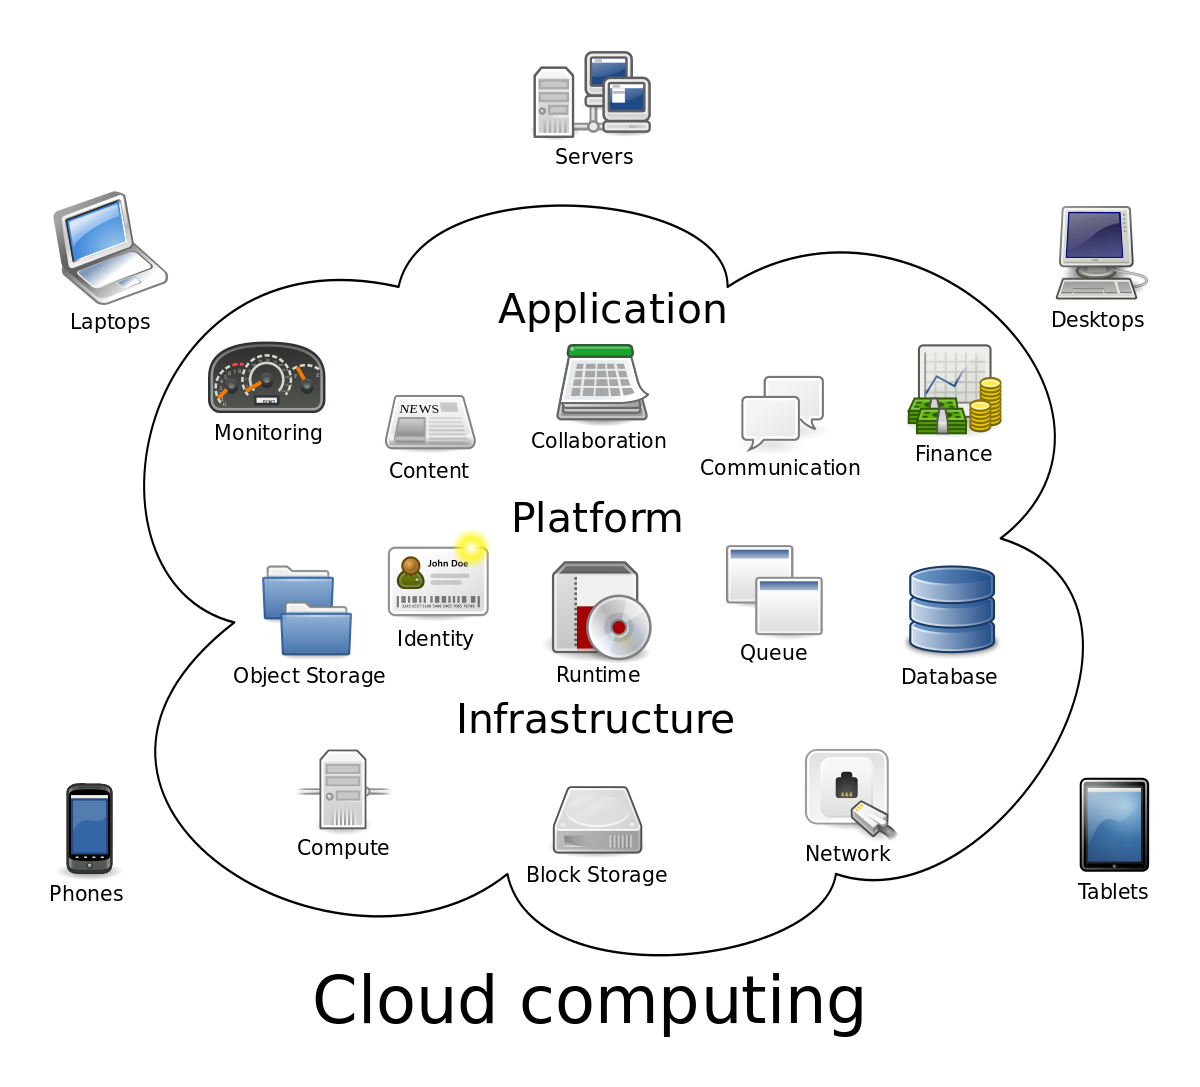
\includegraphics[width=10cm]{texfiles/images/Cloud_computing.png}
 %   \label{fig:cloud_computing_demo}
\newline
Four main models used for deployment of Cloud Computing are as follows \cite{mell62011}:\\
\textbf{Private Cloud:}  It is set up by a single organization for its own use or for customers.\\
\textbf{Community Cloud:} The infrastructure is provided for use by organizations which can have \\multiple customers.\\
\textbf{Public Cloud:} In this kind of deployment model general public is given access to resources in cloud on internet.\\
\textbf{Hybrid Cloud:} A hybrid cloud is a computing environment that combines a public cloud and a private cloud by allowing data and applications to be shared between them.\\
Security Issues with respect to Cloud Computing \cite{fernandes2014security} have been widely discussed both in academics and industry several international conferences have focused on this subject :\\
Confidentiality\\
Virtualization Level Issues\\
Multi Tenancy Issues\\
VM Isolation Issues\\
Virtual Network Issues\\
Virtual Machine Introspection Issues\\
VM Management Issues\\
Application Level Issues\\
Isolation Issues\\
Synchronization Mechanism Issues\\
Data Storage Level Issues\\
Outsourcing Issues\\
Data Deletion Issues\\
Network Level Issues \\
\newline
DoS attacks, and DDOS attacks affect cloud computing infrastructure and services. These type of attacks are major attacks which affect the available services. The Cloud Infrastructure \\provided by vendor could be a victim of such attacks but apart from that it could also be participating in such attacks. Botnets , botClouds can be deployed in Cloud Environment \cite{de2019cyber} to launch such attacks. Hence from security perspective it is important to identify such an issue that may exist in underlying cloud infrastructure.\\
Three main type of service models used in Cloud Computing are as following :\\
Infrastructure as a Service (IaaS)\\
Platform as a Service (PaaS)\\
Software as a Service (SaaS)\\
In \cite{linthicum2017connecting} author discusses that with the advent of cloud computing a lot of data has been generated how this data has been impacting the world and there is a lot of growth in the data of devices that have been connected. So, with the improvements in bandwidth and availability. In the context of the Internet of Things, the trouble with the cloud is that data needs to be sent back from the sensors gathering info, such as a Nest thermostat or a Fitbit wristband, to a database in a remote public cloud. The time that it takes for the data to be transferred from the device or sensor to the remote public cloud, that is the latency, is often too great to meet the requirements of the IoT system. The cloud complicates this process even more.We’re focused on centralized computing, thus there will be latency. Now, instead of sending the data back to the data centre on the other side of the factory, we send it to a remote cloud server that can be thousands of miles away. To make things worse, we send it over the open Internet.\\
In \cite{shen2017block} discussion about data sharing has been made. As how participants must share data. Protocols have played an important role. Protocols have played an important role in transfer of data in case of cloud computing. Storage has become a hot topic in today’s cloud computing world. We prefer to store all types of data in cloud servers, which is also a good option for companies and organizations to avoid the overhead of deploying and maintaining equipment when data are stored locally. In cryptography, a key agreement protocol is a protocol in which two or more parties can agree on a key in such a way that both influence the outcome.  This kind of protocol has widespread application in technology of internet and cloud computing.\\
In \cite{shirazi2017extended} mobile edge computing and emerging models in fog computing have been discussed. Relation between them is evident. The approach in the paper is to examine and underpin the models that are existing in cloud computing. Characteristics of cloud like support of ubiquitous connectivity, elasticity, scalable resources and ease of deployment have played an important role in development of existing cloud computing infrastructure. Research community has proposed new technologies namely fog and cloud. These technologies have been labelled in the paper as extended cloud they allow computing needs to be performed closer to source of data. This results in improvement in quality of services provided since this results in reduction of delay in conveying data between end nodes and cloud. Such technologies have enabled support for new application and services example Google now, foursquare and both are location aware applications for mobile platforms. Further this can be extended to services like autonomous vehicles robotics, public safety and augmented reality.

The acceptable level of service depends upon user expectations. Now these days users require rapid access to service like always on always available. So a new term has popped up known as resilience \cite{shirazi2017extended}. Resilience is concerned with availability of services and maintaining confidentiality and integrity of information in face of challenges. Resilience has become a fundamental property of cloud service provisioning platforms. With the advancement in wireless related technologies security and resiliency have become key issues when considering Mobile Edge Computing Services. With regards to edge model there are few threats also which have evolved. For example, infrastructure related threats, virtualization related threats, privacy related threats.
Fog computing model was originally conceived by Cisco as an extension of cloud. The term fog was originally coined by Cisco as there is need to enable a platform that can cope up with the requirements posed by challenges put forward by Internet of Things. Another requirement in fog computing is privacy of data. In the paper detection and resilience mechanism have been discussed. 
The area that has been challenging to researchers is anomaly detection.
In September 2016 \cite{kolias2017ddos} website of computer security consultant Brian Krebs was hit with 620 Gbps traffic. At the same time a bigger DDoS attack using Mirai malware was done on French web hosting and cloud service provider OVH. Mirai’s source code was release by its creator soon after wards. Hackers offered Mirai’s botnets for rent with as many as 400,000 connected devices. More attacks happened in October 2016 using Mirai they took down hundreds of websites like Twitter,Netflix,Reddit, Github for several hours. Mirai spreads by infecting devices as web cams,DVRs, routers, then it finds out administrative controls of those devices by a brute force attack which relies on a dictionary of potential usernames and passwords.






\clearemptydoublepage
\chapter{First Contribution}
\label{chap:chapter3}
We have studied various anomaly detection techniques deployed by cloud service providers for their services. The study from our side for various cloud service providers for anomaly detection is our first contribution for the project. In this study we took three major service providers Microsoft,Amazon and Google.\\
\section{How Microsoft detects anomaly in azure}
Microsoft uses a technology called security centre\cite{microsf41} in its cloud environments.To detect threats and reduce false positives Security Centre collects data from Azure resources and network and then applies a lot of  machine learning and big data algorithms to detect threat.These techniques as more advance than normal signature based anomaly detection techniques.It is impossible to manually identify the attack and predict the attack when it might happen.So the Microsoft \\ Security Centre uses following technologies\\\\
\textbf{Intelligent threat intelligence} \newline It looks for bad actors by using the information obtained via Microsoft Products and services,Microsoft Digital Crimes Unit and Microsoft Security Response Centre along with external feeds.Microsoft has an immense amount of global threat intelligence. Telemetry flows in from multiple sources, such as Azure, Office 365, Microsoft CRM online, Microsoft Dynamics AX, outlook.com, MSN.com, the Microsoft Digital Crimes Unit (DCU), and Microsoft Security Response Center (MSRC). Researchers also receive threat intelligence information that is shared among major cloud service providers and feeds from other third parties. Azure Security Center can use this information to alert you to threats from known bad actors.\newline \newline
\textbf{Behavioral analytics} \\ Behavioral analytics is a technique that analyzes and compares data to a collection of known patterns. However, these patterns are not simple signatures. They are determined through complex machine learning algorithms that are applied to massive datasets. They are also determined through careful analysis of malicious behaviors by expert analysts. Azure Security Center can use behavioral analytics to identify compromised resources based on analysis of virtual machine logs, virtual network device logs, fabric logs, crash dumps, and other sources.
In addition, there's correlation with other signals to check for supporting evidence of a widespread campaign. This correlation helps to identify events that are consistent with established indicators of compromise.\newline \newline
\textbf{Anomaly detection}\\It uses statistical techniques to build a historical data which is based on usage patterns and any deviation from normal alerts those deviations and it creates a baseline which if confirms to a potential attack vector then the particular usage is detected as an anomaly and in turn thus could be a security event.\newline\newline
Security Centre in Azure also works with connected partner solutions, like firewall and endpoint protection solutions. Microsoft uses \textbf{Fusion Analytics} \cite{mslinks2} as the backbone of Security Centre's anomaly detection system.Fusion works by looking at various kind of alerts generated in Microsoft Azure ecosystem and then it tries to find  pattern which could reveal attack progression indicating what should be next course of action.
\section{How Amazon finds anomalies in AWS}
Amazon uses a technology called guard duty\cite{amazon2}.It is a threat detection service which continuously monitors for bad behavior and protects aws accounts and workloads.In the cloud collection and aggregation of  network activities is simplified, but it can be time consuming for security teams to continuously analyze event log data for potential threats. With the help of GuardDuty now you have an intelligent and cost effective solution to for threat detection in AWS cloud. This technology uses machine learning, anomaly detection, and integrated threat intelligence to identify and prioritize potential threats. GuardDuty analyzes tens of billions of events across multiple AWS data sources, such as AWS CloudTrail, Amazon VPC Flow Logs, and DNS logs. With a few clicks in the AWS Management Console, GuardDuty can be enabled with no software or hardware to deploy or maintain. By integrating with AWS CloudWatch Events, GuardDuty alerts are actionable, easy to aggregate across multiple accounts, and straightforward to push into existing event management and workflow systems.
\section{How Google finds anomalies in GCP cloud }
Google uses an open source library Forseti\cite{google31} which can\\
\begin{itemize}
    \item Detect unusual firewall behaviors between snapshots.
    \item Alert users to any unusual behaviors and provide a comparison with expected behaviors.
    \item Provide potential remediation steps.
\end{itemize}

The key elements for this technology are firewall rules.Firewall rules can be inbound or outbound.A firewall rule can either allow traffic based on IP address or ports.Firewall rules are applied to those instances which are associated with the user who has created his cloud in GCP setup.
The figure below shows the technical architecture as how this has been implemented in GCP \newline


\begin{figure}[h]
    \centering
    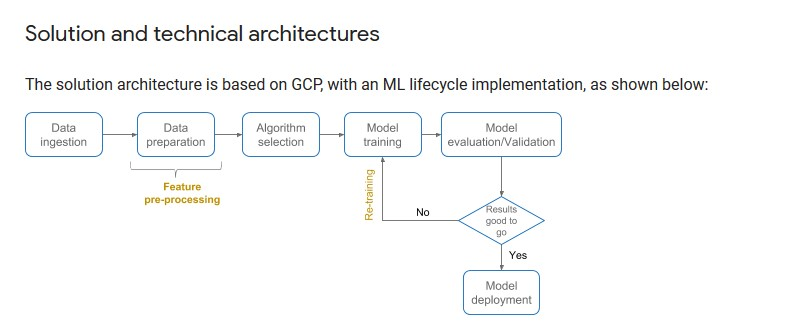
\includegraphics{texfiles/images/gcp_security_model1.jpg}
    \caption{GCP Anomaly Detection}
    \label{fig:GCP Anomaly Detection}
\end{figure}



\clearemptydoublepage
\input{texfiles/Chapter4}
\clearemptydoublepage
\chapter{Conclusion}
\label{chap:conclusion}
%htihktnhkr\cite{12008} \cite{22009}  \cite{32006} \cite{42005} \cite{52007} \cite{62007} 
Anomaly Detection is one of the important security problem in today's world.A significant number of techniques have been developed which are also based on data analytics techniques.So to identify anomaly we have to understand the flow of system and comparing the data sets we can find out pattern in intrusions or attacks. Attack classification and mapping of attack should be done corresponding to each attack.Machine learning techniques have played an important role in finding anomalies in existing systems.Current systems are evolving and getting mature day by day new attacks surface and along with them new techniques are also evolving. Among the existing approaches how can we increase the accuracy of anomaly detection and reduce false positives in cloud computing is an area which will keep attracting researchers in coming years as more and more techniques evolve.
\clearemptydoublepage

%\bibliographystyle{abbrv}
%\clearemptydoublepage
%\singlespace
%\bibliography{biblio}

 
  %\cite{*}
 %\bibliographystyle{plain}
 %\bibliographystyle{alpha}
  \bibliographystyle{unsrt}
  \clearemptydoublepage
  \bibliography{texfiles/bibthesis}
%\addcontentsline{toc}{chapter}{References}

%\input{texfiles/flat}
%\clearemptydoublepage
%\input{texfiles/nest}
%\clearemptydoublepage
%\input{texfiles/intent}
%\clearemptydoublepage
%\input{texfiles/lm}
%\clearemptydoublepage
%\input{texfiles/conclusions}
%\clearemptydoublepage

%\appendix

%\bibliographystyle{abbrv}
%\clearemptydoublepage
%\singlespace
%\bibliography{thesis}

% \include{AppendixA}
% \clearemptydoublepage
% \include{AppendixB}
% \clearemptydoublepage

%\phantomsection \addcontentsline{toc}{chapter}{Index}
%\renewcommand{\baselinestretch}{1} \small \normalsize
 \clearemptydoublepage

\phantomsection \addcontentsline{toc}{chapter}{Author's Biography} %Optional
\chapter*{}
 \begin{center}
 %\hrule height 0.5pt
 {\Huge \bfseries Author's Biography}
 \vspace{1cm}
 %\hrule height 0.5pt
 \end{center}
 
 \onehalfspace
 \noindent author received his B.Tech  degree in Information Technology  from   and Management, in . He has been pursuing M. Tech at the Department of Computer Science and Engineering,  Gati, since Ju 018.
 
 \singlespace
 \begin{center}
 %\hrule height 0.5pt
 \vspace{0.3cm}
 {\bfseries {\large Publications made out of this thesis\\}}
 (listed in reverse chronological order)
 \vspace{0.3cm}
 %\hrule height 0.5pt
 \end{center}
 
 \begin{enumerate}
\item Publication 1 in standard reference format
\item Publication 2 in standard reference format

 	  
 \end{enumerate}

\end{document}

%%%%%%%%%%%%%%%%%%
\if 0

\begin{figure}[tb]
\centerline{
\includegraphics[width=0.5\textwidth]{./figures/}
}
\caption{{\bf }}
\label{fig:}
\end{figure}

\begin{figure*}[tb]
\centerline{
\subfloat[{\bf }]{\includegraphics[height=0.3\textwidth,width=3.5cm,angle=-90]{./figures/}}
\hfil
\subfloat[{\bf }]{\includegraphics[height=0.3\textwidth,width=3.5cm,angle=-90]{./figures/}}
\hfil
\subfloat[{\bf }]{\includegraphics[height=0.3\textwidth,width=3.5cm,angle=-90]{./figures/}}
}
\caption{{\bf }}
\label{fig:}
\end{figure*}

\fi
%%%%%%%%%%%%%%%%%%
